\chapter{Eigenvectors and Eigenvalues of the Moment Covariance Matrix}
\label{ch:lesson06}

In Chapter~\ref{ch:lesson05} we used central moments to find a blob's orientation and, with a bit of extra algebra, its semi-axis lengths. This chapter makes that connection explicit and general: the central moments of \emph{any} blob (not just an ellipse) define a $2\times2$ \textbf{covariance matrix}, and the eigenvectors/eigenvalues of that matrix directly give the orientation and size of the \emph{equivalent ellipse} --- the ellipse with the same area and same second-moment spread as the blob.

\section{Refresher: what are eigenvectors and eigenvalues?}

For a square matrix $A$, a nonzero vector $v$ is an \textbf{eigenvector} with \textbf{eigenvalue} $\lambda$ if
\begin{equation}
Av = \lambda v.
\end{equation}
In words: applying $A$ to $v$ doesn't rotate $v$ off its own line --- it only \emph{scales} it, by a factor of $\lambda$. Most vectors get both rotated and scaled by $A$; eigenvectors are the special directions that only get scaled.

For a $2\times2$ \textbf{symmetric} matrix (like the covariance matrices built below), something even nicer is guaranteed: there are always two eigenvectors, they are perpendicular to each other, and their eigenvalues are real numbers. Geometrically, $A$ takes a circle of unit vectors and stretches it into an ellipse whose axes point along the eigenvectors, with each semi-axis length equal to the corresponding eigenvalue.

\begin{lstlisting}
A = np.array([[3.0, 1.0], [1.0, 1.5]])
eigvals, eigvecs = np.linalg.eigh(A)  # ascending order
\end{lstlisting}

Figure~\ref{fig:l06-1} shows this geometrically.

\begin{figure}[h]
\centering
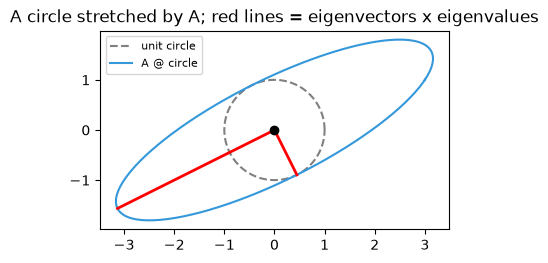
\includegraphics[width=0.42\textwidth]{figures/lesson06_fig01.png}
\caption{A unit circle stretched by $A$; the red lines are the eigenvectors scaled by their eigenvalues.}
\label{fig:l06-1}
\end{figure}

\subsection*{From one eigenvector to both at once: diagonalization}

$Av=\lambda v$ holds for a single eigenvector. Stack \emph{both} eigenvectors as the columns of $P=\begin{bmatrix}v_1 & v_2\end{bmatrix}$, and both eigenvalues on the diagonal of $\Lambda$. Then $Av_1=\lambda_1 v_1$ and $Av_2=\lambda_2 v_2$, side by side, become one matrix equation:
\begin{equation}
AP = P\Lambda.
\end{equation}
Because $A$ is symmetric, its eigenvectors are orthonormal, which makes $P$ an \textbf{orthogonal} matrix ($P^{-1}=P^\top$). That lets us solve for $A$ itself:
\begin{equation}
A = P\Lambda P^\top,
\end{equation}
the \textbf{diagonalization} of $A$. Geometrically this is three steps: $P^\top$ \emph{rotates} coordinates into the eigenvector frame, $\Lambda$ \emph{scales} along those (now axis-aligned) directions independently, and $P$ \emph{rotates back}. When $A$ is a covariance matrix, the off-diagonal entry that mixes $x$ and $y$ is exactly $\mu_{11}$: diagonalizing the covariance matrix and finding the ellipse's own natural axes are the same operation.

\section{From central moments to a covariance matrix}

Treat a blob's pixels as samples from a 2D distribution. Its covariance matrix, in terms of the central moments $\mu_{ij}$ and area $m_{00}$, is
\begin{equation}
A = \frac{1}{m_{00}}\begin{bmatrix}\mu_{20} & \mu_{11} \\ \mu_{11} & \mu_{02}\end{bmatrix}.
\end{equation}
This is exactly the covariance-matrix formula for a scatter of points $(x,y)$, just weighted by pixel membership instead of sample index. Diagonalizing it gives eigenvectors along the blob's own major and minor axes and eigenvalues measuring the spread along each. This same operation, applied to a covariance matrix of general (not necessarily 2D pixel) data, is called \textbf{principal component analysis (PCA)}: the eigenvectors ranked by eigenvalue are the \emph{principal components}, often used to reduce a high-dimensional dataset down to just its most informative few directions.

\begin{lstlisting}
def covariance_from_moments(binary):
    m = cv2.moments(binary, binaryImage=True)
    cx, cy = m['m10'] / m['m00'], m['m01'] / m['m00']
    cov = np.array([[m['mu20'], m['mu11']],
                     [m['mu11'], m['mu02']]]) / m['m00']
    return cov, (cx, cy)
\end{lstlisting}

\section{Eigen decomposition gives orientation and size}

For a filled ellipse with semi-axes $a \ge b$, the eigenvalues of its covariance matrix work out to $\lambda_{\max}=a^2/4$ and $\lambda_{\min}=b^2/4$, so
\begin{equation}
a = 2\sqrt{\lambda_{\max}}, \qquad b = 2\sqrt{\lambda_{\min}},
\end{equation}
with the corresponding eigenvectors pointing along the major and minor axes. The angle of the major axis matches the angle computed from central moments directly in Chapter~\ref{ch:lesson05}.

\begin{lstlisting}
def principal_axes(binary):
    cov, center = covariance_from_moments(binary)
    eigvals, eigvecs = np.linalg.eigh(cov)
    semi_axes = 2 * np.sqrt(np.clip(eigvals, 0, None))
    order = [1, 0]  # largest eigenvalue first
    return center, semi_axes[order], eigvecs[:, order].T
\end{lstlisting}

Figure~\ref{fig:l06-2} confirms the recovered axes against the known ellipse.

\begin{figure}[h]
\centering
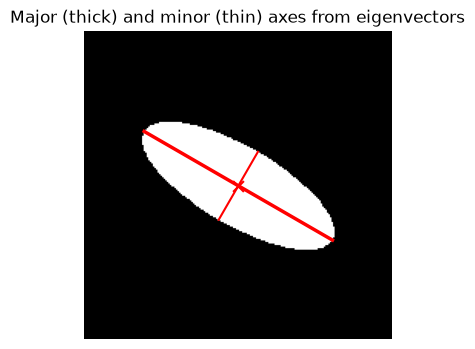
\includegraphics[width=0.4\textwidth]{figures/lesson06_fig02.png}
\caption{Major (thick) and minor (thin) axes recovered from a known ellipse's eigenvectors: $a=70.6$, $b=25.5$, matching the drawn semi-axes (70, 25).}
\label{fig:l06-2}
\end{figure}

\section{It works on arbitrary shapes, too}

The real power of this approach is that it doesn't require the blob to be an ellipse at all. Every binary shape has \emph{some} equivalent ellipse --- the one that matches its area, centroid, and second-moment spread, giving a compact 5-number summary (center, two semi-axis lengths, orientation) of an arbitrarily shaped blob, as in Figure~\ref{fig:l06-3}.

\begin{figure}[h]
\centering
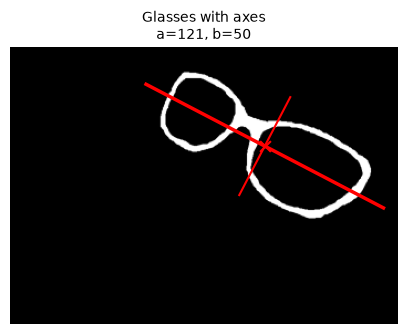
\includegraphics[width=0.42\textwidth]{figures/lesson06_fig03.png}
\caption{Equivalent-ellipse axes for a pair of eyeglasses. The ellipse summarizes the mass distribution rather than tracing the outline, so it cuts across the bridge between lenses. \attrib{Photo: Stan Birchfield.}}
\label{fig:l06-3}
\end{figure}

\section{Eccentricity: how elongated is a shape?}

The ratio of the eigenvalues (or semi-axes) gives a single number describing elongation, independent of orientation and overall size:
\begin{equation}
\text{eccentricity} = \sqrt{1 - \frac{\lambda_{\min}}{\lambda_{\max}}}.
\end{equation}
This ranges from 0 (a circle, both axes equal) to nearly 1 (a very thin, elongated shape). The glasses shape above ($a=120.9$, $b=49.9$) has eccentricity $0.911$ --- clearly elongated, as expected of a pair of glasses lying flat.

\subsection*{Exercises}
\begin{enumerate}
  \item Draw a perfect circle and confirm its eccentricity is (close to) 0.
  \item Overlay the \emph{actual} fitted ellipse outline (not just the axis lines) using \code{cv2.ellipse} with the center, \code{(2a, 2b)} as the full axes lengths, and the orientation angle from the eigenvectors. Compare it to \code{cv2.fitEllipse} applied to the shape's contour --- do they agree?
  \item Run \code{principal\_axes} on the filled blob of the glasses (after flood fill). How much do $a$, $b$, and the eccentricity change? Does that match your intuition for how moments depend on \emph{where} mass sits, not just the overall silhouette?
\end{enumerate}

\vfill
\fullcode{lesson06}{lesson06_eigen_covariance}
